\documentclass[11pt,a4paper]{article}
\usepackage[utf8]{inputenc}
\usepackage[T1]{fontenc}
\usepackage[spanish,es-nodecimaldot]{babel}
\usepackage{lmodern,microtype,amsmath,amssymb,booktabs,longtable,array,graphicx,float,xcolor}
\usepackage[margin=2.25cm,headheight=15pt]{geometry}
\usepackage{fancyhdr,enumitem}
\usepackage[colorlinks=true,linkcolor=teal!65!black,urlcolor=teal!65!black,citecolor=teal!65!black]{hyperref}
\definecolor{azul}{HTML}{193B50}
\definecolor{verde}{HTML}{087E8B}
\setlength{\parindent}{0pt}
\setlength{\parskip}{6pt}
\setlength{\emergencystretch}{2em}
\setlist{itemsep=2pt,topsep=4pt}
\pagestyle{fancy}
\fancyhf{}\fancyhead[L]{\small Modelos matemáticos de la ciencia II}
\fancyhead[R]{\small Regresión múltiple}\fancyfoot[C]{\thepage}
\renewcommand{\headrulewidth}{0.3pt}
\hypersetup{pdftitle={Regresión múltiple aplicada al tiempo de un solver disperso},pdfauthor={Informe académico}}
\newcommand{\W}{X_2}\newcommand{\V}{X_3}
\makeatletter
\renewcommand{\l@section}{\@dottedtocline{1}{0em}{2em}}
\makeatother
\begin{document}
\hypersetup{pageanchor=false}
\begin{titlepage}
\vspace*{1.7cm}
{\color{verde}\large COMPUTACIÓN CIENTÍFICA\par}
\vspace{0.7cm}
{\color{azul}\Huge\bfseries Regresión lineal\par múltiple\par}
\vspace{0.8cm}
{\LARGE Estimación del tiempo de ejecución\par de un solver de sistemas dispersos\par}
\vspace{0.7cm}
{\large Ejercicio propuesto y solución completa\par}
\vspace{1.3cm}
\rule{\linewidth}{0.6pt}
\textbf{Curso:} Modelos matemáticos de la ciencia II\\
\textbf{Área:} Escuela Profesional de Computación Científica\\
\textbf{Material principal:} Semana 9 y extracto de regresión múltiple del proyecto del curso.\\
\textbf{Fecha:} 28 de octubre de 2026\par
\rule{\linewidth}{0.6pt}
\vfill
\colorbox{verde!8}{\parbox{.94\linewidth}{\textbf{Naturaleza del ejercicio.} Los 48 registros son simulados con semilla fija. Se analiza un escenario de benchmarking; no se presentan mediciones de hardware real. El HTML complementario funciona sin conexión y conserva el mismo modelo del informe.}}
\end{titlepage}
\hypersetup{pageanchor=true}

\section*{Resumen}
Se propone un problema reproducible de predicción del tiempo de un solver iterativo disperso. Las regresoras son el trabajo acumulado sobre elementos no nulos y el volumen escrito en puntos de control. Se generan 48 observaciones, de las cuales 36 se destinan a estimación y 12 a prueba. Mediante mínimos cuadrados ordinarios (MCO) se obtiene
\[
\widehat T=1.414171+0.160782W+1.385309V.
\]
El ajuste alcanza $R^2=0.9792$ y un error estándar residual de $0.6036$ segundos. En prueba, el RMSE es $0.5707$ segundos. Se desarrollan las operaciones de estimación, ANOVA, inferencia individual y conjunta, análisis de residuos, validación y simulación. Los resultados son coherentes con el mecanismo generador; su uso en otro equipo requeriría mediciones y validación adicionales.

\textbf{Criterio de presentación.} Se escribe primero el problema y luego se resuelve, mostrando fórmula, sustitución, decisión e interpretación, siguiendo el enfoque del curso. Se usa $\beta_1$ como intercepto y $\beta_2,\beta_3$ como pendientes, igual que en la semana 9 \cite{semana9,extracto}.
\begingroup\small\setlength{\parskip}{0pt}\tableofcontents\endgroup
\newpage

\section{Planteamiento del problema}
\subsection*{Enunciado del ejercicio}
Un laboratorio utiliza un solver iterativo para resolver sistemas lineales dispersos $A\boldsymbol z=\boldsymbol b$. Necesita estimar el tiempo total de un lote antes de programarlo en una estación de trabajo. El algoritmo y el equipo se mantienen fijos. En cada lote se conoce el número total de elementos no nulos procesados durante las iteraciones y el volumen escrito como puntos de control o \emph{checkpoints}.

Se dispone de 48 registros simulados. Para cada registro se observan el tiempo total $T$ en segundos, el trabajo $W$ en millones de elementos no nulos procesados y el volumen escrito $V$ en GB decimales. Los registros 1--36 se reservan para ajuste y los registros 37--48 para prueba. Con $\alpha=0.05$:
\begin{enumerate}
\item Formular y estimar un modelo de regresión múltiple de $T$ respecto de $W$ y $V$; interpretar sus coeficientes.
\item Calcular residuos, evaluar ajuste y supuestos, y realizar contrastes individuales y globales.
\item Validar el modelo sin utilizar los datos de prueba para ajustar parámetros.
\item Predecir el tiempo cuando $W=60$ millones y $V=2.5$ GB, con intervalos del 95\%.
\item Simular ajustes repetidos y construir una herramienta interactiva que permita probar el modelo.
\end{enumerate}

\subsection*{Justificación computacional y alcance}
En un método disperso, el costo acumulado depende del trabajo efectivamente procesado. Si una matriz tiene $m$ elementos no nulos y se ejecutan $q$ iteraciones con un recorrido de la matriz por iteración, entonces $W=mq/10^6$. Por ejemplo, $m=10^6$ y $q=60$ producen $W=60$. Si cada iteración requiere varios recorridos, se deben contabilizar todos. Los demás costos que escalan de forma estable con ese trabajo quedan absorbidos en el coeficiente efectivo.

La entrada y salida aporta otro costo que se aproxima por una tasa efectiva constante. El modelo es una aproximación aditiva para una implementación y un rango acotados. No describe cambios de complejidad, saturación de memoria, comunicación entre nodos o superposición variable entre cómputo y escritura. Su objetivo es didáctico y predictivo dentro del escenario simulado, sin atribuir causalidad empírica.

\section{Recolección y presentación de datos}
\subsection{Diccionario de variables y unidad de observación}
La unidad de observación es un lote completo de ejecución, con su trabajo total y volumen total. $Y=T$ es cuantitativa continua de razón. $X_2=W$ es una medida de conteo escalada, y $X_3=V$ es cuantitativa continua de razón.
\begin{center}
\begin{tabular}{p{1.8cm}p{7.3cm}p{3.2cm}}\toprule
Símbolo & Definición operativa & Unidad\\\midrule
$Y_i=T_i$ & Tiempo de cómputo y escritura del lote & segundos\\
$X_{2i}=W_i$ & Trabajo acumulado sobre no nulos & millones de elementos\\
$X_{3i}=V_i$ & Volumen total de checkpoints escritos & GB ($10^9$ bytes)\\\bottomrule
\end{tabular}
\end{center}

\subsection{Origen reproducible de los registros}
Se usa \texttt{numpy.random.default\_rng(20261028)}. En este orden se generan 48 enteros uniformes $W\in\{20,\ldots,100\}$, 48 enteros uniformes $J\in\{5,\ldots,45\}$ y se define $V=J/10$. Luego se generan 48 errores independientes normales de desviación $0.55$ segundos:
\[
T_i=\operatorname{redondear}_{0.001}\left(2+0.16W_i+1.20V_i+u_i\right),
\qquad u_i\overset{\mathrm{iid}}\sim N(0,0.55^2).
\]
Los coeficientes del generador se conocen para evaluar la simulación, pero \textbf{no se usan para estimar el modelo}. El pequeño redondeo introduce una diferencia despreciable respecto de una normal exacta. No se eligió una semilla buscando que las pruebas aprobaran. El orden de generación se conserva como orden de ejecución simulado.

La partición 36/12 se fija antes del ajuste. No hay valores faltantes. Los valores se conservaron como fueron generados, sin eliminar observaciones. El archivo \texttt{datos\_y\_residuos.csv} y el anexo A contienen los 48 registros. En las 36 filas de ajuste los rangos efectivos son $W\in[21.0,100.0]$ y $V\in[0.6,4.5]$.
\begin{center}
\begin{tabular}{lrrrr}\toprule
Variable & Media & Desviación muestral & Mínimo & Máximo\\\midrule
Trabajo $W$ & 54.472 & 24.089 & 21.000 & 100.000\\
Volumen $V$ & 2.492 & 1.173 & 0.600 & 4.500\\
Tiempo $T$ & 13.624 & 4.067 & 6.186 & 21.599\\
\bottomrule\end{tabular}
\end{center}
La correlación de Pearson entre las regresoras es $r_{WV}=-0.1148$. Esta correlación describe el diseño; no es una prueba de causalidad.

\subsection{Protocolo propuesto para recolectar datos reales}
Para sustituir la simulación por mediciones: fijar equipo, solver, precondicionador, número de hilos y versiones; registrar frecuencia y condiciones térmicas; hacer calentamientos fuera del cronometraje; variar $W$ y $V$ con orden aleatorio; medir el tiempo con un reloj monotónico de alta resolución; sincronizar al terminar la escritura para evitar medir solo el búfer; repetir cada configuración y conservar las repeticiones individuales. Definir expresamente si se incluye inicialización. Se deben registrar fallos de convergencia y cargas externas, y justificar cualquier exclusión antes de analizar resultados. Si hay agrupamientos por sesión, las particiones de validación deben respetarlos.

\section{Formulación del modelo matemático}
La función de regresión poblacional es
\begin{equation}
Y_i=\beta_1+\beta_2X_{2i}+\beta_3X_{3i}+u_i,
\qquad E(u_i\mid X_{2i},X_{3i})=0.
\end{equation}
Así, $E(Y_i\mid W_i,V_i)=\beta_1+\beta_2W_i+\beta_3V_i$. Se estiman $k=3$ parámetros con $n=36$ filas de ajuste y quedan $n-k=33$ grados de libertad. En notación matricial,
\[
\boldsymbol y=X\boldsymbol\beta+\boldsymbol u,\quad
X=\begin{bmatrix}1&W_1&V_1\\\vdots&\vdots&\vdots\\1&W_{36}&V_{36}\end{bmatrix},
\quad\boldsymbol\beta=\begin{bmatrix}\beta_1\\\beta_2\\\beta_3\end{bmatrix}.
\]
Se espera $\beta_2>0$ y $\beta_3>0$, aunque los contrastes se plantean bilateralmente. El modelo es lineal en los parámetros y usa una variable de trabajo que ya incorpora la interacción entre no nulos e iteraciones. La normalidad de los errores se añade para la inferencia exacta clásica, pero no es necesaria para calcular MCO.

\section{Estimación de los coeficientes de regresión}
\subsection{Función objetivo y ecuaciones normales}
MCO minimiza
\[
Q(\boldsymbol\beta)=\sum_{i=1}^{36}(Y_i-\beta_1-\beta_2W_i-\beta_3V_i)^2.
\]
Derivando: $\partial Q/\partial\beta_1=-2\sum\hat u_i=0$, $\partial Q/\partial\beta_2=-2\sum W_i\hat u_i=0$ y $\partial Q/\partial\beta_3=-2\sum V_i\hat u_i=0$. Por tanto,
\[
X^{\mathsf T}X\widehat{\boldsymbol\beta}=X^{\mathsf T}\boldsymbol y,
\qquad \widehat{\boldsymbol\beta}=(X^{\mathsf T}X)^{-1}X^{\mathsf T}\boldsymbol y.
\]
Los productos obtenidos exclusivamente con las 36 filas de ajuste son
\[
X^{\mathsf T}X=\begin{bmatrix}36.000 & 1961.000 & 89.700\\1961.000 & 127129.000 & 4772.600\\89.700 & 4772.600 & 271.690\end{bmatrix},\qquad
X^{\mathsf T}\boldsymbol y=\begin{bmatrix}490.465\\29824.713\\1270.572\end{bmatrix}.
\]
El rango de $X$ es 3. Para computar se utiliza la solución por pseudoinversa basada en SVD de \texttt{statsmodels.OLS}, evitando resolver el problema mediante una inversión explícita de las ecuaciones normales. La inversa se muestra para explicar la teoría y obtener las varianzas.

\subsection{Solución mediante desviaciones respecto de las medias}
Sean $w_i=W_i-\bar W$, $v_i=V_i-\bar V$ y $y_i=Y_i-\bar Y$. Las medias son $\bar W=54.472222$, $\bar V=2.491667$ y $\bar Y=13.624028$. Se calculan
\begin{align*}
S_{ww}=\sum w_i^2&=20308.972222,& S_{vv}=\sum v_i^2&=48.187500,\\
S_{wv}=\sum w_iv_i&=-113.558333,& S_{wy}=\sum w_iy_i&=3107.994528,\\
S_{vy}=\sum v_iy_i&=48.496508.
\end{align*}
Al eliminar el intercepto quedan $S_{ww}\hat\beta_2+S_{wv}\hat\beta_3=S_{wy}$ y $S_{wv}\hat\beta_2+S_{vv}\hat\beta_3=S_{vy}$. Con $D=S_{ww}S_{vv}-S_{wv}^2=965743.103889>0$:
\begin{align*}
\hat\beta_2&=\frac{S_{wy}S_{vv}-S_{vy}S_{wv}}{D}
=\frac{(3107.994528)(48.187500)-(48.496508)(-113.558333)}{965743.103889}=0.160782,\\
\hat\beta_3&=\frac{S_{vy}S_{ww}-S_{wy}S_{wv}}{D}
=\frac{(48.496508)(20308.972222)-(3107.994528)(-113.558333)}{965743.103889}=1.385309,\\
\hat\beta_1&=\bar Y-\hat\beta_2\bar W-\hat\beta_3\bar V\\
&=13.624028-(0.160782)(54.472222)-(1.385309)(2.491667)=1.414171.
\end{align*}
Las cifras mostradas están redondeadas; los cálculos de archivos y aplicación utilizan precisión completa.

\section{Ecuación de regresión obtenida}
\begin{equation}\boxed{\widehat T=1.414171+0.160782W+1.385309V\quad\text{segundos}.}\end{equation}
Manteniendo $V$ fijo, un millón adicional de elementos no nulos procesados se asocia con $0.160782$ segundos más. Un aumento de diez millones se asocia con $1.6078$ segundos. Manteniendo $W$ fijo, cada GB adicional escrito se asocia con $1.385309$ segundos más.

El intercepto es el tiempo estimado en $W=V=0$, punto fuera del dominio observado. Por ello se interpreta como un parámetro de ajuste y no como una medición del costo de arranque del equipo. La pendiente de escritura equivale a una tasa efectiva aproximada de $1/\hat\beta_3=0.7219$ GB/s; se trata de una interpretación del escenario simulado, no de una especificación real del disco.

\section{Cálculo y evaluación de residuos}
Para las filas de ajuste, $\hat u_i=Y_i-\widehat Y_i$. Un residuo positivo indica que el tiempo observado superó al estimado. Para la primera observación:
\begin{align*}
\widehat T_1&=1.414171+(0.160782)(33.000000)+(1.385309)(4.500000)=12.953854,\\
\hat u_1&=12.300000-12.953854=-0.653854\text{ s},\qquad \hat u_1^2=0.427525\text{ s}^2.
\end{align*}
La suma de cuadrados residual es
\[
SC_{\mathrm{res}}=\sum_{i=1}^{36}\hat u_i^2=12.0247,\quad
\hat\sigma^2=\frac{SC_{\mathrm{res}}}{36-3}=0.364385,\quad s=\sqrt{\hat\sigma^2}=0.6036\text{ s}.
\]
Se verifica $\sum\hat u_i\simeq0$ y $X^{\mathsf T}\hat{\boldsymbol u}\simeq\boldsymbol0$ numéricamente. Son identidades de MCO con intercepto; no demuestran la exogeneidad ni la media condicional cero del error poblacional.

Para comparar residuos con distinta precisión se calculan
\[
h_i=\boldsymbol x_i^{\mathsf T}(X^{\mathsf T}X)^{-1}\boldsymbol x_i,\quad
r_i=\frac{\hat u_i}{s\sqrt{1-h_i}},\quad
D_i=\frac{r_i^2}{k}\frac{h_i}{1-h_i}.
\]
$r_i$ es el residuo estandarizado interno y $D_i$ la distancia de Cook. El máximo $|r_i|$ es $1.9971$, el máximo leverage es $0.1595$ y la máxima distancia de Cook es $0.2165$. No hay filas con $|r_i|>2$ ni con $h_i>2k/n=0.1667$. Las filas 2, 12, 24, 31 superan $4/n=0.1111$ en Cook. Estos cortes son señales de revisión, no reglas automáticas de eliminación.

Se hizo un análisis de sensibilidad exploratorio retirando conjuntamente esas cuatro filas: las pendientes se vuelven $0.161449$ y $1.288247$, con cambios relativos de $0.41\%$ y $-7.01\%$. Las diferencias merecen reportarse, aunque el signo positivo se conserva. El modelo principal mantiene todas las observaciones. La prueba reservada no se usa para decidir exclusiones ni seleccionar esta variante.

\section{Evaluación del ajuste del modelo}
Definimos sin ambigüedad $SC_{\mathrm{tot}}=\sum(Y_i-\bar Y)^2$, $SC_{\mathrm{reg}}=\sum(\widehat Y_i-\bar Y)^2$ y $SC_{\mathrm{res}}=\sum\hat u_i^2$. Con intercepto,
\[
SC_{\mathrm{tot}}=SC_{\mathrm{reg}}+SC_{\mathrm{res}}
=566.8908+12.0247=578.9155.
\]
\begin{align*}
R^2&=1-\frac{SC_{\mathrm{res}}}{SC_{\mathrm{tot}}}=1-\frac{12.0247}{578.9155}=0.9792,\\
\bar R^2&=1-\frac{SC_{\mathrm{res}}/(n-k)}{SC_{\mathrm{tot}}/(n-1)}=0.9780.
\end{align*}
El modelo explica el $97.92\%$ de la variabilidad observada en el conjunto de ajuste. El RMSE de ajuste es $0.5779$ s y el MAE $0.4642$ s. El RMSE usa divisor $n$; el error estándar $s$ usa divisor $n-k$. No son la misma cantidad. Un $R^2$ alto no garantiza predicciones correctas fuera del diseño ni valida los supuestos por sí solo.
\begin{figure}[H]\centering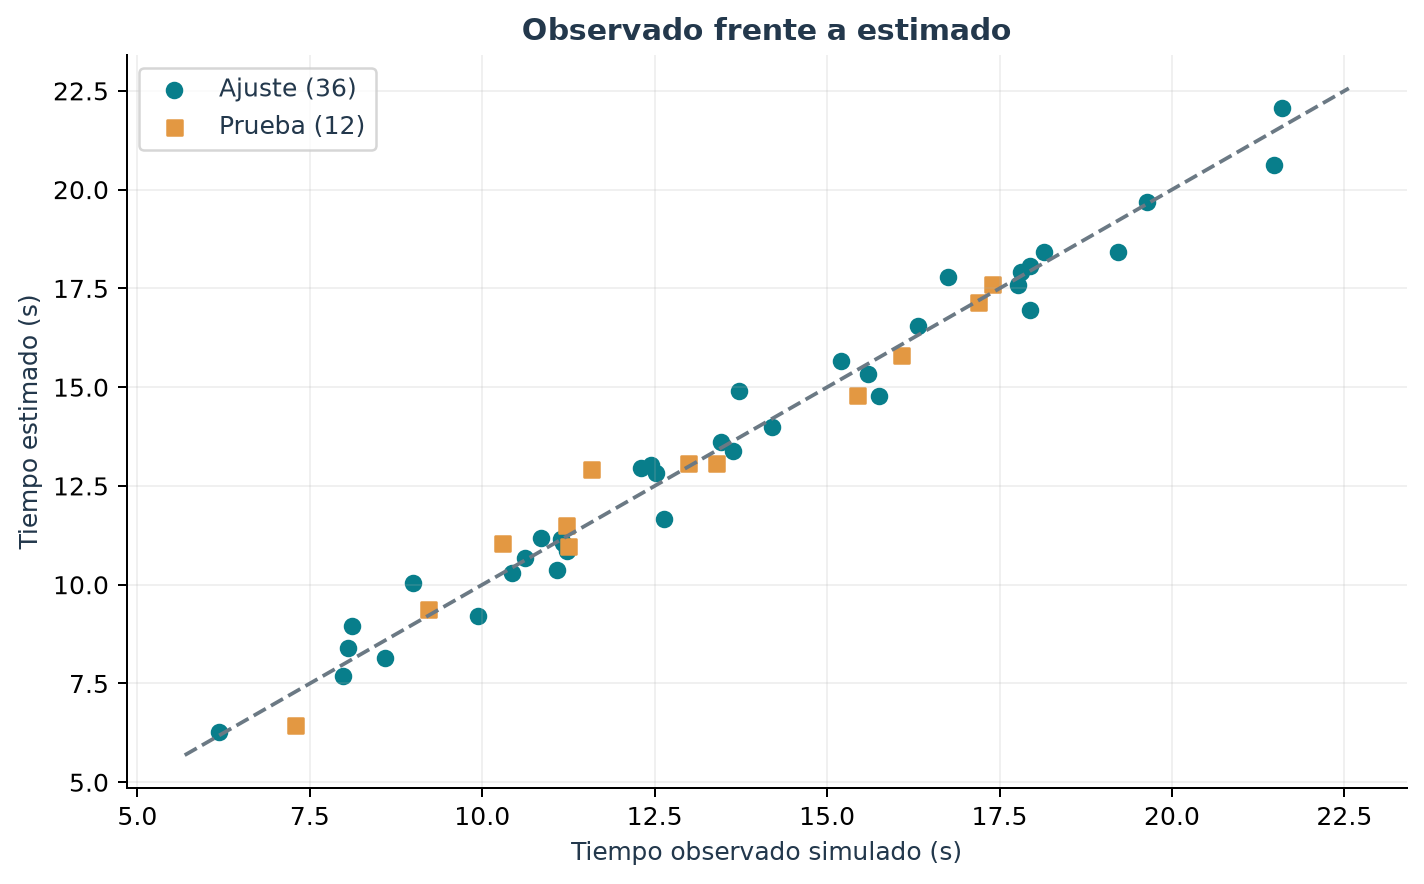
\includegraphics[width=.84\linewidth]{images/ajuste.png}\caption{Comparación de tiempos observados simulados y estimados. La línea discontinua representa predicción perfecta.}\end{figure}

\section{Evaluación de los supuestos del modelo}
\begin{enumerate}
\item \textbf{Linealidad y especificación.} Se justifican por la suma de costos de trabajo y escritura. Se inspeccionan residuos frente a ajustados y a cada regresora. RESET explora una desviación cuadrática, pero no descarta toda omisión o interacción posible.
\item \textbf{Exogeneidad y media condicional cero.} Son condiciones del generador porque el ruido se produce independientemente de $W,V$. En un benchmark real exigirían control experimental; los residuos por sí solos no las verifican.
\item \textbf{Homoscedasticidad.} El generador usa varianza constante; se contrasta con la versión de Koenker de la prueba de Breusch--Pagan y se revisa la dispersión residual. Se comparan además errores estándar HC3.
\item \textbf{Independencia.} El ruido se genera independientemente. Se usa el orden conservado de ejecución para revisar autocorrelación de primer orden; no se ordenan las filas por $W$ o $V$ antes del contraste. Ausencia de autocorrelación no implica independencia general.
\item \textbf{Variación y no colinealidad perfecta.} $n=36>k=3$, las dos regresoras varían y $\operatorname{rango}(X)=3$. Para dos regresoras $VIF=1/(1-r_{WV}^2)=1.0134$ en ambas pendientes, sin evidencia de inflación fuerte. En modelos con más regresoras se usa el $R_j^2$ de cada regresión auxiliar.
\item \textbf{Normalidad de los errores.} Es parte de la simulación antes del redondeo, y se evalúa mediante Q-Q, Shapiro--Wilk y Jarque--Bera. La normalidad interesa para inferencia clásica exacta; no implica normalidad de $W,V$ o de los tiempos marginales.
\end{enumerate}
Los residuos de MCO están correlacionados a través de la matriz $I-H$ y tienen varianza $\sigma^2(1-h_i)$. Por ello, las pruebas sobre residuos son diagnósticos aproximados; no deben confundirse con observación directa de errores iid. Los gráficos no muestran curvatura ni un embudo marcado, y el orden no exhibe una tendencia persistente.
\begin{figure}[H]\centering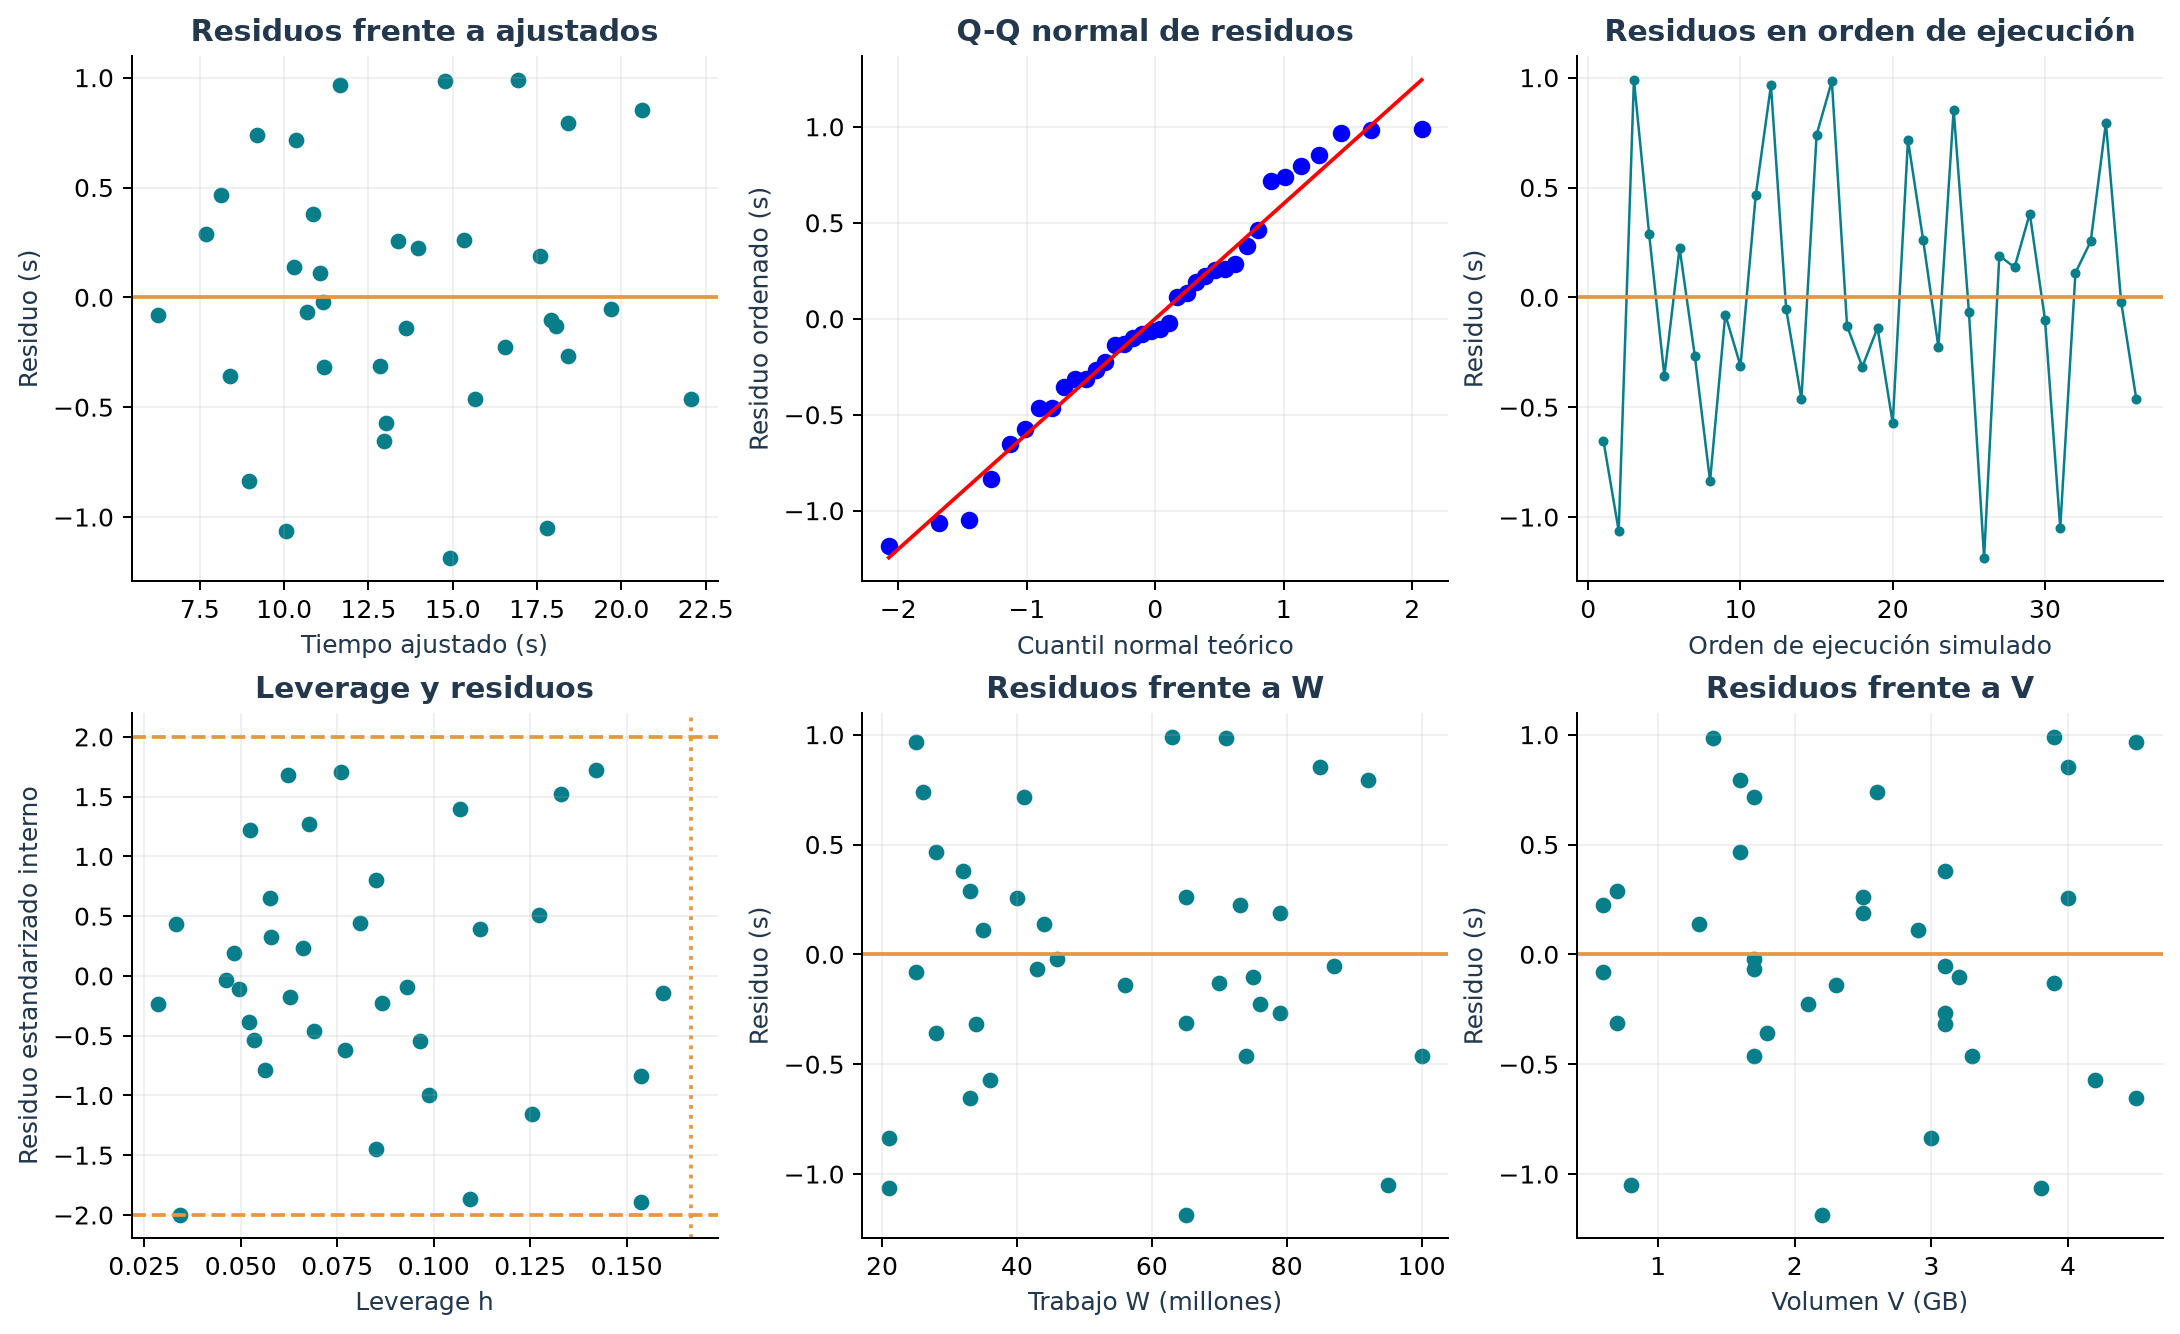
\includegraphics[width=\linewidth]{images/diagnosticos.png}\caption{Diagnósticos con las 36 filas de ajuste. Las líneas de leverage y residuos son umbrales orientativos.}\end{figure}

\section{Pruebas estadísticas de los residuos}
En cada prueba se fija $\alpha=0.05$: se rechaza la hipótesis nula cuando $p<0.05$. Los valores $p$ no son probabilidades de que $H_0$ sea verdadera. Los diagnósticos se interpretan en conjunto con el diseño y los gráficos \cite{nist,statsmodels}.
\begin{center}\small
\begin{tabular}{p{5.1cm}rrp{3.5cm}}\toprule
Prueba & Estadístico & $p$ & Decisión al 5\%\\\midrule
Shapiro-Wilk & 0.9703 & 0.4340 & No rechazar $H_0$\\
Jarque-Bera & 0.5286 & 0.7677 & No rechazar $H_0$\\
Koenker/Breusch--Pagan & 1.1869 & 0.5524 & No rechazar $H_0$\\
Breusch-Godfrey, orden 1 & 0.0189 & 0.8908 & No rechazar $H_0$\\
RESET, potencia 2 & 0.0438 & 0.8356 & No rechazar $H_0$\\
\bottomrule\end{tabular}\end{center}
\textbf{Normalidad.} Shapiro--Wilk contrasta compatibilidad con una distribución normal. Jarque--Bera usa asimetría $S$ y curtosis $K$:
\[
JB=\frac{n}{6}\left(S^2+\frac{(K-3)^2}{4}\right)\ \dot\sim\ \chi^2_2.
\]
Ambos valores $p$ exceden 0.05. No se detecta evidencia de no normalidad; no se demuestra que la distribución sea normal.

\textbf{Varianza constante.} La versión robusta de Koenker de Breusch--Pagan regresa $\hat u_i^2$ sobre $1,W_i,V_i$ y calcula $LM=nR^2_{\mathrm{aux}}\dot\sim\chi^2_2$. Se obtiene $LM=1.1869$ y $p=0.5524$. No se rechaza homoscedasticidad. Se especifica esta versión para distinguirla de la formulación original sensible a normalidad \cite{bpdoc}.

\textbf{Correlación serial.} Breusch--Godfrey de orden 1 incorpora el residuo rezagado a la regresión auxiliar, conservando el orden de ejecución; $H_0:\rho_1=0$ y $LM\dot\sim\chi^2_1$. El resultado es $LM=0.0189$, $p=0.8908$. Durbin--Watson es $1.9018$ y se presenta como descripción complementaria, sin atribuirle un valor $p$ calculado. No se detecta autocorrelación de primer orden \cite{bgdoc}.

\textbf{Especificación.} RESET añade $\widehat Y_i^2$ al modelo y contrasta que su coeficiente sea cero mediante $F_{1,32}$. El resultado $F=0.0438$, $p=0.8356$ no indica necesidad de ese término. Puede haber otras formas de especificación incorrecta no detectadas. Las cinco pruebas son exploratorias, sin corrección por multiplicidad; su potencia es limitada con 36 registros.

\section{Pruebas de hipótesis de los coeficientes de regresión}
Para $j=1,2,3$: $H_0:\beta_j=0$ frente a $H_1:\beta_j\ne0$. Se estima
\[
\widehat{\operatorname{Var}}(\widehat{\boldsymbol\beta})
=s^2(X^{\mathsf T}X)^{-1},\quad
t_j=\frac{\hat\beta_j}{ee(\hat\beta_j)},\quad
IC_{95\%}(\beta_j)=\hat\beta_j\pm t_{0.975,33}\,ee(\hat\beta_j).
\]
Aquí $t_{0.975,33}=2.0345$. Se rechaza $H_0$ si $|t_j|>2.0345$ o si el valor $p$ bilateral es menor que 0.05.
\begin{center}\small
\begin{tabular}{lrrrrr}\toprule
Parámetro & Estimación & Error est. & $t$ & $p$ & IC 95\%\\\midrule
$\beta_{1}$ & 1.414171 & 0.351106 & 4.0278 & $0.0003$ & $[0.6998,2.1285]$\\
$\beta_{2}$ & 0.160782 & 0.004264 & 37.7068 & $1.031\times10^{-28}$ & $[0.1521,0.1695]$\\
$\beta_{3}$ & 1.385309 & 0.087537 & 15.8253 & $5.682\times10^{-17}$ & $[1.2072,1.5634]$\\
\bottomrule\end{tabular}\end{center}
Las dos pendientes son significativas y positivas. El intercepto también resulta significativo, pero ello no valida una interpretación física fuera del rango. Las pruebas individuales se interpretan como inferencia nominal al 5\%, sin ajuste para contrastes múltiples. Como control de sensibilidad a heteroscedasticidad, los errores estándar HC3 son $(0.294287,0.004984,0.098330)$; las dos pendientes conservan $p<0.05$ con HC3.

\section{Prueba de hipótesis global del modelo}
La hipótesis global es $H_0:\beta_2=\beta_3=0$ frente a que al menos una pendiente sea distinta de cero. El intercepto no forma parte de esta restricción. La tabla ANOVA es
\begin{center}
\begin{tabular}{lrrrr}\toprule
Fuente & Suma de cuadrados & gl & Cuadrado medio & $F$\\\midrule
Regresión & 566.8908 & 2 & 283.4454 & 777.8729\\
Residuos & 12.0247 & 33 & 0.364385 & \\
Total & 578.9155 & 35 & & \\\bottomrule
\end{tabular}\end{center}
\[
F=\frac{SC_{\mathrm{reg}}/2}{SC_{\mathrm{res}}/33}
=\frac{283.4454}{0.364385}=777.8729
\quad\overset{H_0}{\sim}\quad F_{2,33}.
\]
El valor crítico es $F_{0.95;2,33}=3.2849$ y $p=1.730\times10^{-28}$. Como $F$ excede el valor crítico, se rechaza $H_0$: el modelo completo aporta explicación lineal respecto de un modelo con solo intercepto. Esto no significa que todos los supuestos estén demostrados ni que cada variable deba ser significativa individualmente; esa última conclusión requiere sus pruebas t.

\section{Validación del modelo}
\subsection{Estrategia sin fuga de información}
Las 12 filas de prueba permanecen fuera de la estimación, diagnósticos y selección. Sobre las 36 filas de ajuste se ejecuta validación cruzada de seis particiones: se permutan sus índices con semilla 20261029, se forman seis grupos de seis y cada grupo se predice con un modelo ajustado con las otras 30 filas. Cada fila obtiene una predicción fuera de su ajuste. No se eligieron variables ni hiperparámetros usando estos resultados.
\[
RMSE=\sqrt{\frac1m\sum_{i=1}^m(Y_i-\widehat Y_i)^2},\qquad
MAE=\frac1m\sum_{i=1}^m|Y_i-\widehat Y_i|.
\]
Para cada conjunto se usa $R^2=1-\sum(Y-\widehat Y)^2/\sum(Y-\bar Y_{\mathrm{conjunto}})^2$. La media de referencia de $R^2$ es la del conjunto evaluado; la predicción del modelo base, en cambio, es la media del entrenamiento correspondiente.
\begin{center}\begin{tabular}{lrrr}\toprule
Evaluación & RMSE (s) & MAE (s) & $R^2$\\\midrule
Ajuste (36) & 0.5779 & 0.4642 & 0.9792\\
Cruzada, fuera de ajuste (36) & 0.6100 & 0.4816 & 0.9769\\
Base, cruzada (36) & 4.0622 & 3.4355 & -0.0262\\
Prueba reservada (12) & 0.5707 & 0.4360 & 0.9658\\
Base, prueba (12) & 3.2017 & 2.7825 & -0.0762\\
\bottomrule\end{tabular}\end{center}
Los resultados por partición son los siguientes. Las métricas agregadas anteriores se calculan juntando los 36 errores fuera de ajuste, no promediando los seis $R^2$.
\begin{center}\begin{tabular}{lrrr}\toprule
Partición & $m$ & RMSE (s) & MAE (s)\\\midrule
1 & 6 & 0.4753 & 0.3066\\
2 & 6 & 0.7830 & 0.6574\\
3 & 6 & 0.7288 & 0.6465\\
4 & 6 & 0.5550 & 0.4363\\
5 & 6 & 0.6836 & 0.5871\\
6 & 6 & 0.2949 & 0.2554\\
\bottomrule\end{tabular}\end{center}

\subsection{Interpretación de la prueba reservada}
El RMSE de prueba es $0.5707$ s, frente a $3.2017$ s del modelo base. El MAE de prueba es $0.4360$ s, y $R^2_{\mathrm{prueba}}=0.9658$. La cercanía con validación cruzada ($RMSE=0.6100$ s) no sugiere una degradación grande en esta pequeña reserva. Los intervalos de predicción del 95\% incluyen 11 de los 12 tiempos observados ($91.67\%$). Esta fracción pequeña no permite estimar con precisión la cobertura real ni demostrar una cobertura nominal del 95\%.

Se conserva el modelo ajustado con 36 filas para mantener idénticos coeficientes en el informe y el HTML. No se reajusta con las 48 filas después de evaluar. En un proyecto real haría falta una validación independiente por sesión, equipo y régimen de trabajo; una partición aleatoria dentro de una misma máquina no garantiza transportabilidad.

\section{Predicción mediante el modelo}
Para $W_0=60$ y $V_0=2.5$, $\boldsymbol x_0=(1,60,2.5)^{\mathsf T}$:
\[
\widehat T_0=1.414171+(0.160782)(60)+(1.385309)(2.5)=14.5243\text{ s}.
\]
El factor de varianza es $h_0=\boldsymbol x_0^{\mathsf T}(X^{\mathsf T}X)^{-1}\boldsymbol x_0=0.029315$. El error estándar para la media es $s\sqrt{h_0}=0.1034$ s. Por tanto,
\begin{align*}
IC_{95\%}\{E(T_0\mid\boldsymbol x_0)\}
&=\widehat T_0\pm t_{0.975,33}s\sqrt{h_0}\\
&=14.5243\pm(2.0345)(0.1034)=[14.3141,14.7346]\text{ s}.
\end{align*}
Para una nueva ejecución individual se suma la variabilidad del nuevo error:
\begin{align*}
IP_{95\%}(T_{0,\mathrm{nuevo}})
&=\widehat T_0\pm t_{0.975,33}s\sqrt{1+h_0}\\
&=[13.2783,15.7703]\text{ s}.
\end{align*}
El intervalo individual es más amplio porque incluye incertidumbre sobre la media y fluctuación de una nueva ejecución. Son intervalos frecuentistas, condicionales al modelo y sus supuestos. No incluyen cambios de hardware o errores de especificación. El punto propuesto pertenece a la envolvente convexa del diseño de ajuste. El HTML distingue puntos dentro de esa envolvente, dentro de rangos marginales pero fuera de ella, y fuera de los rangos de ajuste; no recorta silenciosamente entradas ni intervalos.

\section{Simulación y visualización}
\subsection{Experimento Monte Carlo reproducible}
Para separar la variación de una muestra de la conducta repetida del estimador se conserva $X$ de ajuste y se simulan $B=5000$ vectores de tiempos con $\boldsymbol\beta^*=(2,0.16,1.20)^{\mathsf T}$ y $\sigma^*=0.55$, usando semilla 20261030. En esta simulación auxiliar no se redondean los tiempos. Para cada repetición:
\begin{enumerate}
\item Generar $\boldsymbol u^{(b)}\sim N(\boldsymbol0,0.55^2I)$ y definir $\boldsymbol Y^{(b)}=X\boldsymbol\beta^*+\boldsymbol u^{(b)}$.
\item Estimar $\hat{\boldsymbol\beta}^{(b)}$ por MCO y $s_b^2=SC_{\mathrm{res},b}/33$.
\item Construir los tres intervalos t del 95\% y registrar si contienen el valor generador correspondiente.
\item Resumir medias, desviaciones y coberturas empíricas.
\end{enumerate}
\begin{center}\begin{tabular}{lrrrr}\toprule
Coeficiente & Valor generador & Media MCO & DE entre ajustes & Cobertura 95\%\\\midrule
$\beta_{1}$ & 2.000000 & 2.000498 & 0.319906 & 0.9484\\
$\beta_{2}$ & 0.160000 & 0.160054 & 0.003863 & 0.9488\\
$\beta_{3}$ & 1.200000 & 1.198708 & 0.080508 & 0.9470\\
\bottomrule\end{tabular}\end{center}
Las medias estimadas son cercanas a los valores generadores. Las coberturas están próximas a 0.95, coherentes con el modelo normal correcto. La desviación Monte Carlo de una cobertura cercana al 95\% es aproximadamente $\sqrt{0.95(0.05)/5000}=0.0031$, por lo que diferencias de unas décimas de punto porcentual son esperables. Este experimento verifica el procedimiento bajo condiciones conocidas, no la validez física del escenario.
\begin{figure}[H]\centering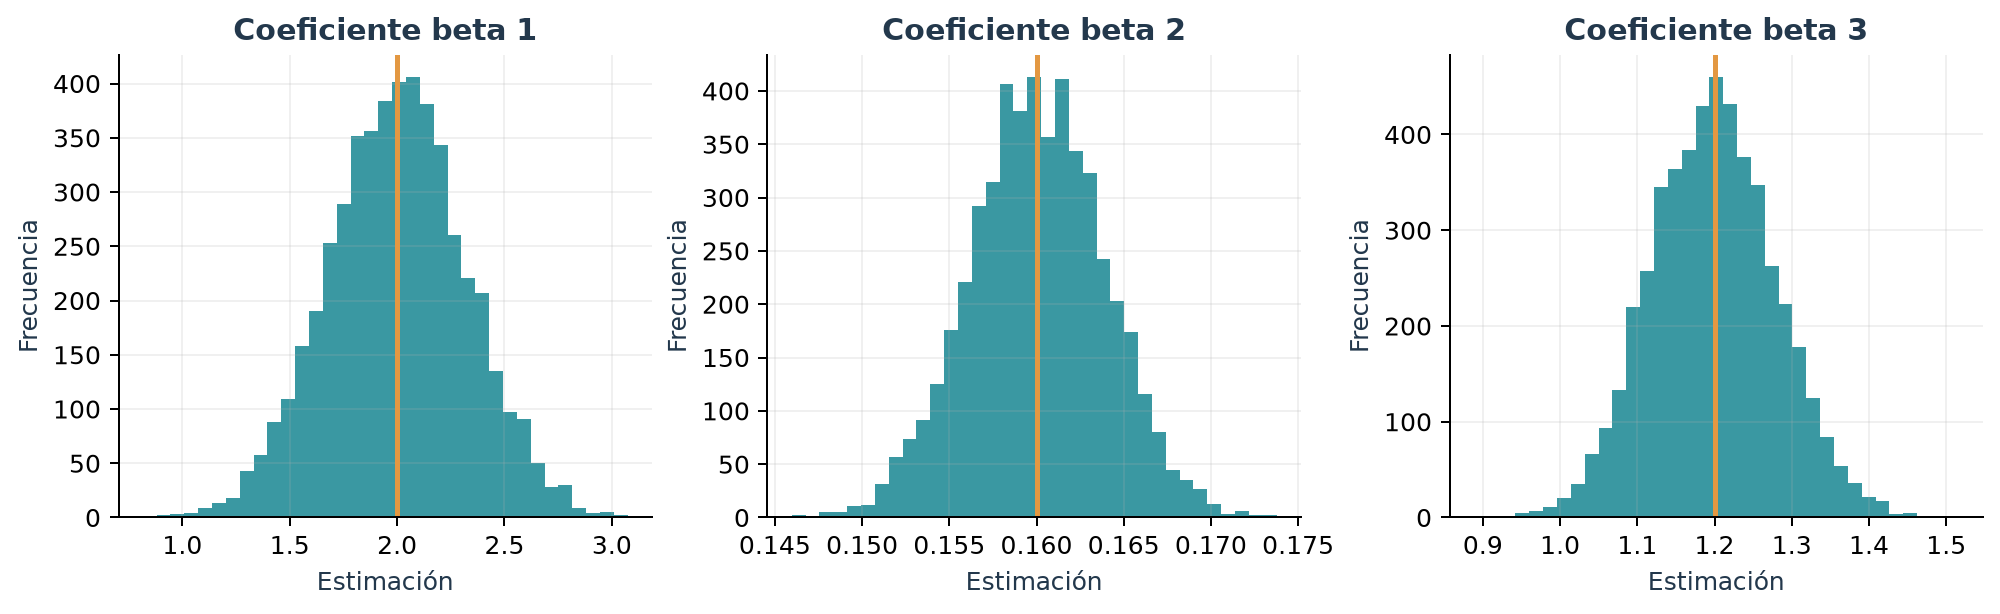
\includegraphics[width=\linewidth]{images/simulacion.png}\caption{Distribución de los coeficientes en 5000 muestras; la línea vertical señala el parámetro generador.}\end{figure}
\begin{figure}[H]\centering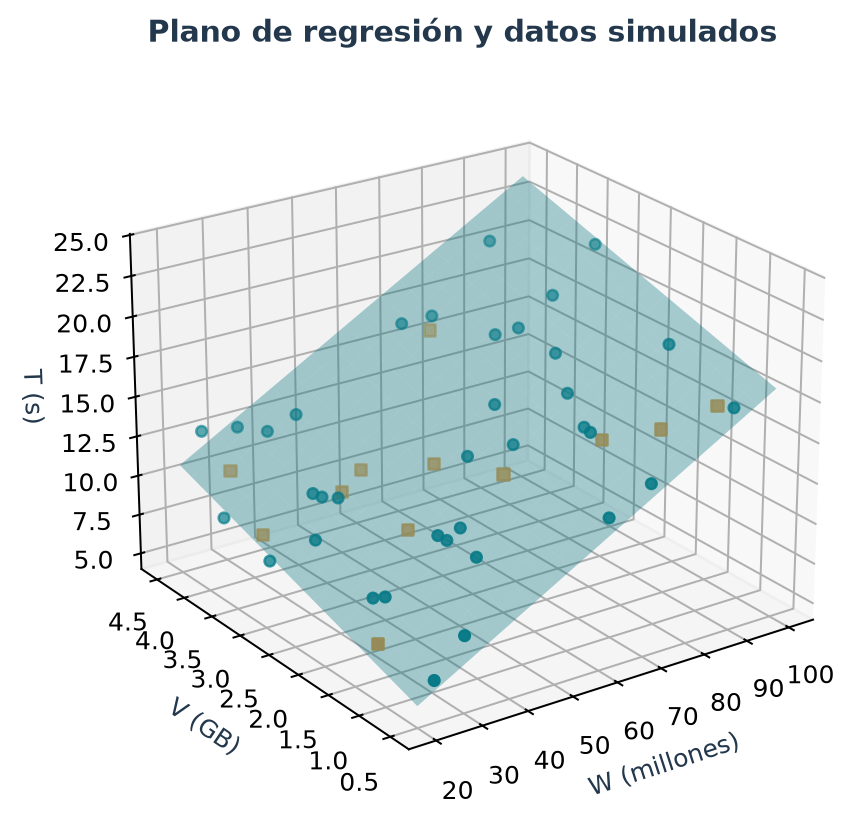
\includegraphics[width=.84\linewidth]{images/plano.png}\caption{Plano estimado: trabajo, volumen y tiempo. Verde: ajuste; naranja: prueba.}\end{figure}

\subsection{Uso de la aplicación HTML}
Abrir \texttt{modelo\_interactivo.html} en un navegador. El archivo es autónomo, sin bibliotecas remotas ni servidor. Permite modificar $W,V$, consultar predicción e intervalos, visualizar la respuesta al variar $W$ con $V$ fijo, inspeccionar diagnósticos, ver todos los registros y descargar un CSV.

La sección de simulación permite cambiar una semilla y $\sigma$, generar otra muestra sobre el mismo diseño y volver a estimar MCO. Se informa el modelo simulado y su RMSE respecto de esa muestra. La simulación del navegador usa su propio generador determinista y Box--Muller; no pretende reproducir la secuencia PCG64 de NumPy. El experimento de 5000 repeticiones del informe se reproduce con el script Python. La muestra interactiva no modifica los coeficientes oficiales usados en predicción, tablas o diagnósticos. Así se distingue la simulación exploratoria del resultado evaluado.

\section{Análisis y discusión de resultados}
El trabajo acumulado y la escritura tienen asociaciones positivas claras con el tiempo. La estimación de trabajo ($0.160782$ s/millón) es cercana al valor generador de 0.16; la de escritura ($1.385309$ s/GB) difiere del 1.20 generador por variación muestral. Una muestra concreta no recupera exactamente parámetros poblacionales. El intercepto también fluctúa y no debe interpretarse físicamente en el origen sin datos allí.

El buen ajuste y los errores fuera de muestra pequeños son esperables porque los datos se generaron con una relación lineal de bajo ruido. Esto hace útil el ejemplo para aprender el procedimiento, pero limita cualquier afirmación sobre rendimiento de un equipo real. La ausencia de rechazos en diagnósticos no equivale a verificar todos los supuestos. La revisión de Cook muestra observaciones cuyo peso conviene discutir; suprimirlas por mejorar resultados produciría un análisis sesgado.

En mediciones reales puede crecer la varianza con la carga, aparecer dependencia térmica o cambiar la tasa de disco. Frente a heteroscedasticidad se revisarían HC3, transformaciones o mínimos cuadrados ponderados justificados; frente a dependencia, un diseño por bloques y métodos apropiados; frente a curvatura, términos adicionales justificados y validados. No se deben añadir términos solo para elevar $R^2$. Al aumentar hilos, cambiar arquitectura o extrapolar fuera del diseño, habría que recolectar nuevos datos.

\section{Conclusiones}
\begin{enumerate}
\item Se resolvió un ejercicio de regresión múltiple con interpretación computacional, estimando tres parámetros a partir de 36 observaciones simuladas y reservando 12 para prueba.
\item La ecuación $\widehat T=1.414171+0.160782W+1.385309V$ presenta pendientes positivas y significativas. El contraste global rechaza pendientes nulas simultáneas.
\item El ajuste obtiene $R^2=0.9792$ y $s=0.6036$ s. Los diagnósticos no detectan las desviaciones específicas contrastadas al 5\%, pero no demuestran los supuestos. Se revisaron cuatro filas con influencia orientativa.
\item La validación cruzada obtiene RMSE de $0.6100$ s y la prueba reservada $0.5707$ s. El ejemplo de $W=60,V=2.5$ produce $14.5243$ s, con IP del 95\% $[13.2783,15.7703]$ s.
\item La simulación repetida apoya la consistencia del cálculo bajo el modelo generador. Antes de utilizar la ecuación en planificación real deben recolectarse benchmarks y validarse el entorno y el dominio de predicción.
\end{enumerate}

\clearpage\section{Referencias bibliográficas}
\begingroup\raggedright\renewcommand{\section}[2]{}\begin{thebibliography}{9}
\bibitem{semana9} Fiestas Flores, R. C. (s. f.). \emph{Semana 9. Regresión lineal múltiple: MCO, ANOVA, coeficientes y supuestos del modelo}. Material del curso Modelos matemáticos de la ciencia II, Escuela Profesional de Computación Científica. Archivo \texttt{9.pdf}, 19 páginas, del proyecto de ChatGPT proporcionado por el usuario. Se consultaron especialmente las páginas 4--18.
\bibitem{extracto} \emph{Regresión Multiple.pdf} (s. f.). Extracto de texto sobre regresión múltiple, 224 páginas. Material del proyecto del curso proporcionado por el usuario. Se consultaron los capítulos 7 y 8 para estimación e inferencia, y el apartado sobre Breusch--Pagan para heteroscedasticidad. El fragmento no incluye portada editorial; se conserva su título de archivo sin inventar metadatos bibliográficos.
\bibitem{nist} NIST/SEMATECH. (s. f.). \emph{e-Handbook of Statistical Methods: Check of assumptions}. \url{https://itl.nist.gov/div898/handbook/pri/section2/pri245.htm}. Consulta: 28 de octubre de 2026.
\bibitem{statsmodels} Proyecto statsmodels. (s. f.). \emph{Regression diagnostics and specification tests}. \url{https://www.statsmodels.org/stable/diagnostic.html}. Consulta: 28 de octubre de 2026.
\bibitem{bpdoc} Proyecto statsmodels. (s. f.). \emph{het\_breuschpagan: Breusch--Pagan Lagrange Multiplier test for heteroscedasticity}. \url{https://www.statsmodels.org/stable/generated/statsmodels.stats.diagnostic.het_breuschpagan.html}. Consulta: 28 de octubre de 2026.
\bibitem{bgdoc} Proyecto statsmodels. (s. f.). \emph{acorr\_breusch\_godfrey: Breusch--Godfrey Lagrange Multiplier tests for residual autocorrelation}. \url{https://www.statsmodels.org/stable/generated/statsmodels.stats.diagnostic.acorr_breusch_godfrey.html}. Consulta: 28 de octubre de 2026.
\end{thebibliography}\endgroup

\appendix\newpage
\section{Datos completos y residuos}
Las filas 1--36 son de ajuste: su diferencia observado menos estimado es un residuo. Las filas 37--48 son de prueba: la diferencia es un error de predicción fuera de muestra. Las cifras se muestran a tres decimales. El CSV incluye además leverage, residuos estandarizados, Cook e intervalos a mayor precisión. Los diagnósticos de influencia solo se definen aquí para las filas usadas en el ajuste.
\small
\begin{longtable}{rllrrrr}
\caption{Los 48 registros y su estimación con el mismo modelo.}\\
\toprule ID & Conjunto & $W$ & $V$ & $T$ & $\widehat T$ & $T-\widehat T$\\\midrule\endfirsthead
\toprule ID & Conjunto & $W$ & $V$ & $T$ & $\widehat T$ & $T-\widehat T$\\\midrule\endhead
1 & ajuste & 33 & 4.5 & 12.300 & 12.954 & -0.654\\
2 & ajuste & 21 & 3.8 & 8.992 & 10.055 & -1.063\\
3 & ajuste & 63 & 3.9 & 17.936 & 16.946 & 0.990\\
4 & ajuste & 33 & 0.7 & 7.977 & 7.690 & 0.287\\
5 & ajuste & 28 & 1.8 & 8.052 & 8.410 & -0.358\\
6 & ajuste & 73 & 0.6 & 14.207 & 13.982 & 0.225\\
7 & ajuste & 79 & 3.1 & 18.144 & 18.410 & -0.266\\
8 & ajuste & 21 & 3.0 & 8.110 & 8.947 & -0.837\\
9 & ajuste & 25 & 0.6 & 6.186 & 6.265 & -0.079\\
10 & ajuste & 65 & 0.7 & 12.523 & 12.835 & -0.312\\
11 & ajuste & 28 & 1.6 & 8.597 & 8.133 & 0.464\\
12 & ajuste & 25 & 4.5 & 12.633 & 11.668 & 0.965\\
13 & ajuste & 87 & 3.1 & 19.643 & 19.697 & -0.054\\
14 & ajuste & 74 & 1.7 & 15.204 & 15.667 & -0.463\\
15 & ajuste & 26 & 2.6 & 9.937 & 9.196 & 0.741\\
16 & ajuste & 71 & 1.4 & 15.753 & 14.769 & 0.984\\
17 & ajuste & 70 & 3.9 & 17.941 & 18.072 & -0.131\\
18 & ajuste & 34 & 3.1 & 10.859 & 11.175 & -0.316\\
19 & ajuste & 56 & 2.3 & 13.465 & 13.604 & -0.139\\
20 & ajuste & 36 & 4.2 & 12.448 & 13.021 & -0.573\\
21 & ajuste & 41 & 1.7 & 11.078 & 10.361 & 0.717\\
22 & ajuste & 65 & 2.5 & 15.588 & 15.328 & 0.260\\
23 & ajuste & 76 & 2.1 & 16.316 & 16.543 & -0.227\\
24 & ajuste & 85 & 4.0 & 21.476 & 20.622 & 0.854\\
25 & ajuste & 43 & 1.7 & 10.618 & 10.683 & -0.065\\
26 & ajuste & 65 & 2.2 & 13.728 & 14.913 & -1.185\\
27 & ajuste & 79 & 2.5 & 17.769 & 17.579 & 0.190\\
28 & ajuste & 44 & 1.3 & 10.426 & 10.289 & 0.137\\
29 & ajuste & 32 & 3.1 & 11.235 & 10.854 & 0.381\\
30 & ajuste & 75 & 3.2 & 17.804 & 17.906 & -0.102\\
31 & ajuste & 95 & 0.8 & 16.747 & 17.797 & -1.050\\
32 & ajuste & 35 & 2.9 & 11.171 & 11.059 & 0.112\\
33 & ajuste & 40 & 4.0 & 13.641 & 13.387 & 0.254\\
34 & ajuste & 92 & 1.6 & 19.217 & 18.423 & 0.794\\
35 & ajuste & 46 & 1.7 & 11.145 & 11.165 & -0.020\\
36 & ajuste & 100 & 3.3 & 21.599 & 22.064 & -0.465\\
37 & prueba & 25 & 4.0 & 11.238 & 10.975 & 0.263\\
38 & prueba & 41 & 2.2 & 10.287 & 11.054 & -0.767\\
39 & prueba & 72 & 1.3 & 15.435 & 14.791 & 0.644\\
40 & prueba & 91 & 0.8 & 17.182 & 17.154 & 0.028\\
41 & prueba & 37 & 3.0 & 11.210 & 11.519 & -0.309\\
42 & prueba & 81 & 1.0 & 16.072 & 15.823 & 0.249\\
43 & prueba & 21 & 1.2 & 7.285 & 6.453 & 0.832\\
44 & prueba & 51 & 2.5 & 12.982 & 13.077 & -0.095\\
45 & prueba & 57 & 1.8 & 13.385 & 13.072 & 0.313\\
46 & prueba & 44 & 3.2 & 11.579 & 12.922 & -1.343\\
47 & prueba & 22 & 3.2 & 9.218 & 9.384 & -0.166\\
48 & prueba & 68 & 3.8 & 17.389 & 17.611 & -0.222\\
\bottomrule\end{longtable}\normalsize

\section{Intervalos y errores en la prueba reservada}
Los límites son intervalos de predicción individuales nominales del 95\%, calculados con $t_{33}$ y varianza de una nueva observación. No son intervalos simultáneos para todas las filas.
\begin{center}\small\begin{tabular}{rrrrrr}\toprule
ID & $T$ & $\widehat T$ & Error & Límite inferior & Límite superior\\\midrule
37 & 11.238 & 10.975 & 0.263 & 9.682 & 12.268\\
38 & 10.287 & 11.054 & -0.767 & 9.802 & 12.306\\
39 & 15.435 & 14.791 & 0.644 & 13.522 & 16.061\\
40 & 17.182 & 17.154 & 0.028 & 15.842 & 18.465\\
41 & 11.210 & 11.519 & -0.309 & 10.263 & 12.775\\
42 & 16.072 & 15.823 & 0.249 & 14.534 & 17.111\\
43 & 7.285 & 6.453 & 0.832 & 5.148 & 7.758\\
44 & 12.982 & 13.077 & -0.095 & 11.832 & 14.323\\
45 & 13.385 & 13.072 & 0.313 & 11.821 & 14.323\\
46 & 11.579 & 12.922 & -1.343 & 11.668 & 14.175\\
47 & 9.218 & 9.384 & -0.166 & 8.105 & 10.664\\
48 & 17.389 & 17.611 & -0.222 & 16.337 & 18.886\\
\bottomrule\end{tabular}\end{center}

\section{Trazabilidad, notación y reproducción}
\textbf{Relación con los materiales.} Se adopta la FRP/FRM con intercepto $\beta_1$, las fórmulas MCO en desviaciones de la página 10 de \texttt{9.pdf}, la varianza residual con $n-k$, VIF, determinación, pruebas t y F. El extracto \texttt{Regresión Multiple.pdf} respalda la interpretación parcial y la inferencia. La validación reservada, los diagnósticos programados y el laboratorio HTML amplían el ejercicio solicitado.

\textbf{Aclaraciones de consistencia.} En las diapositivas 14 y 16 de \texttt{9.pdf} se intercambian los símbolos SCE y SCR entre algunas expresiones. En este informe se definen explícitamente $SC_{\mathrm{reg}}$ y $SC_{\mathrm{res}}$; siempre $R^2=SC_{\mathrm{reg}}/SC_{\mathrm{tot}}$ y $F=(SC_{\mathrm{reg}}/2)/(SC_{\mathrm{res}}/33)$. La derivada parcial correcta de $\beta_2$ en la diapositiva 11 es respecto de $X_2$. En VIF, lo relevante es $|r|\to1$, pues una correlación no puede ser mayor que 1. Finalmente, se escribe ``no rechazar'' una hipótesis en lugar de ``aceptarla'' como verdad demostrada.

\textbf{Reproducción del cálculo.} Ejecutar \texttt{reproducir.py} desde la carpeta del paquete. Se requieren NumPy, SciPy, pandas, statsmodels y Matplotlib. La orden \texttt{python reproducir.py} crea la carpeta \texttt{recalculado/} con datos, resultados y figuras; no altera los entregables originales. Versiones usadas: numpy 2.5.4, scipy 1.18.1, statsmodels 0.15.0, pandas 3.1.0, matplotlib 3.11.2. El script deja fijadas las semillas 20261028 (datos), 20261029 (particiones) y 20261030 (Monte Carlo). \texttt{resultados.json} conserva cifras con precisión completa. El HTML contiene una copia de esos mismos resultados.

\textbf{Compilación.} El archivo principal es \texttt{informe/main.tex}; cargarlo con la carpeta \texttt{images/} en un proyecto de LaTeX y compilar con pdfLaTeX, dos veces para resolver el índice y referencias. También puede usarse Tectonic. No se necesitan archivos bibliográficos externos. El PDF compilado permite revisar el documento sin instalar LaTeX.
\end{document}
